\section{Results}

\subsection{Population density vs Twitter popularity}

To answer our first research question computed the Twitter popularity (or representation) as the number of unique twitter users divided by the population for each municipality. The plot of these values against the population density of 
each municipality is shown on Figure \ref{mun_pop}. The negative correlation observed on the plot is a very surprising result given that the results in the literature show the exact opposite effect. After checking the data thoroughly observed certain anomalies; e.g. a tweet populatity more than 100\% (this is usually very small municipalities which are maybe ski resorts so there are a lot of tweets by people who don't actually live there). We hypothesised that the result may be due the municipalities being too small and adding a lot of noise, so we decided to perform the same analysis on a cantonal level, but the results were even more extreme (see Figure \ref{can_pop}).

\begin{figure}[h]
  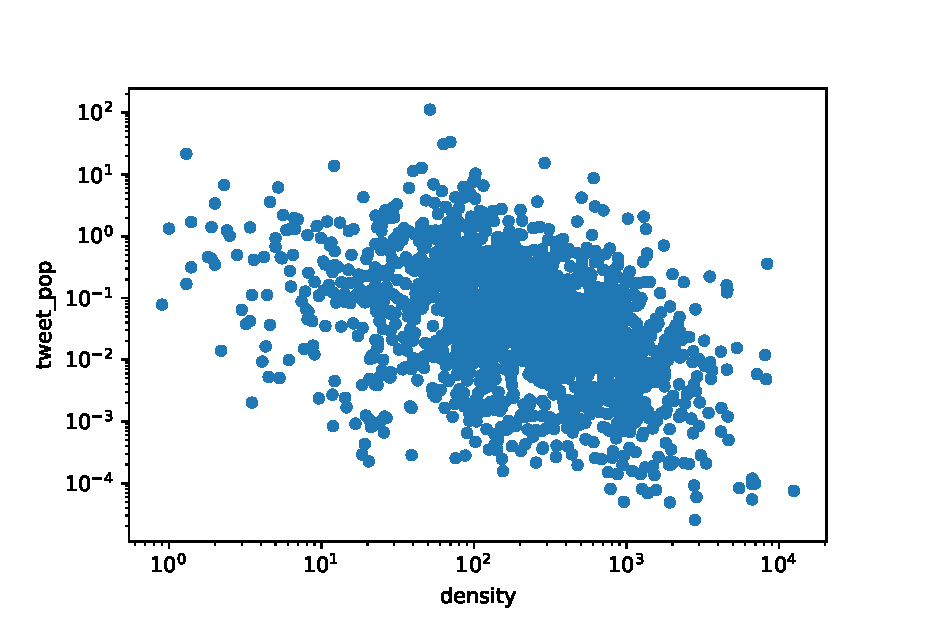
\includegraphics[width=0.5\textwidth]{images/mun_density_pop.eps}
  \caption{We plot the population density vs twitter popularity in each municipality on a log-log scale. The correlation value (of the log values) was -0.398908.}
  \label{mun_pop}
\end{figure}


\begin{figure}[h]
  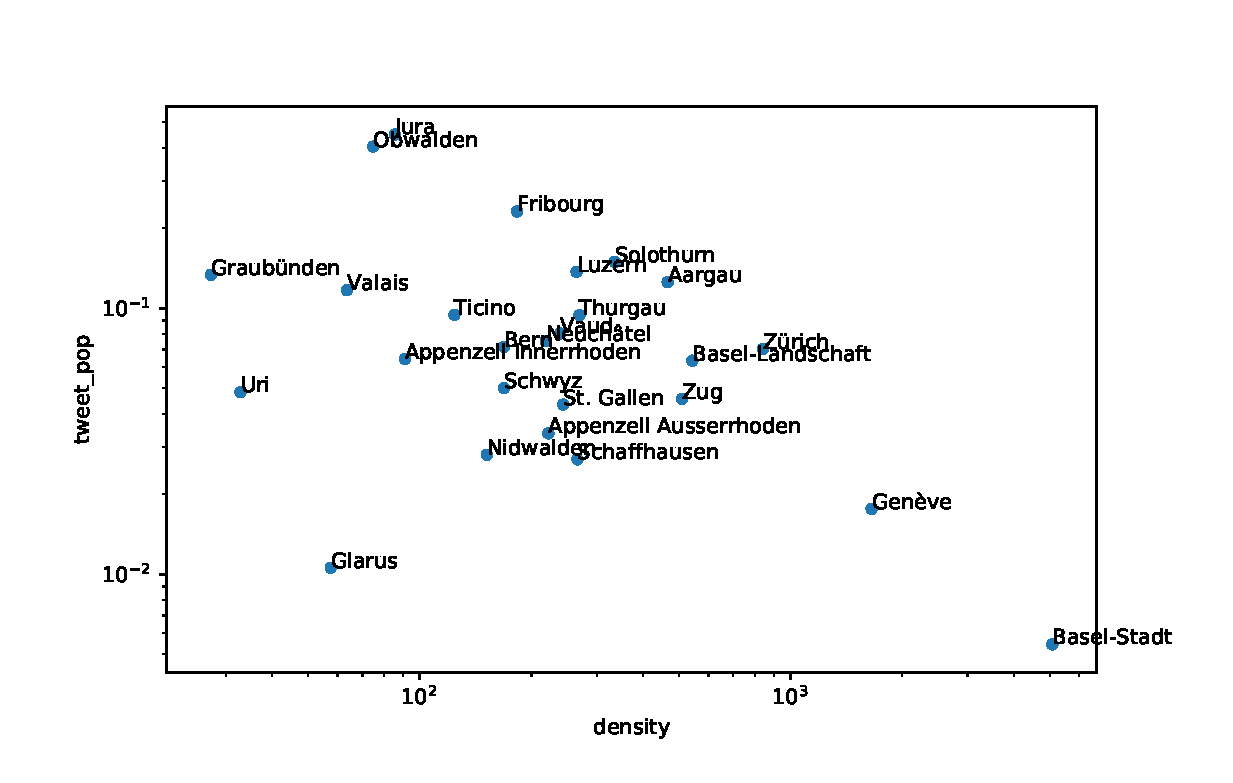
\includegraphics[width=0.5\textwidth]{images/can_density_pop.eps}
  \caption{We plot the population density vs twitter popularity in each canton on a log-log scale. The correlation value (of the log values) was -0.448168.}
  \label{can_pop}
\end{figure}


%%%%%%%%%%%%%%%%%%%%%%%%%%%%%%%
\subsection{Reconstructing the R\"ostigraben}
To detect the R\"ostigraben, we first exlcuded all English language tweets, then we computed the language which had the highest number of tweets for each municipality. We visualize the results on Figure \ref{rosti_map}. Our results seams very robust and agrees with the official definiton of the R\"ostigraben. This is a very reassuring results given the simplicity of our method and our preliminary concerns with the dataset.

\begin{figure}[h]
  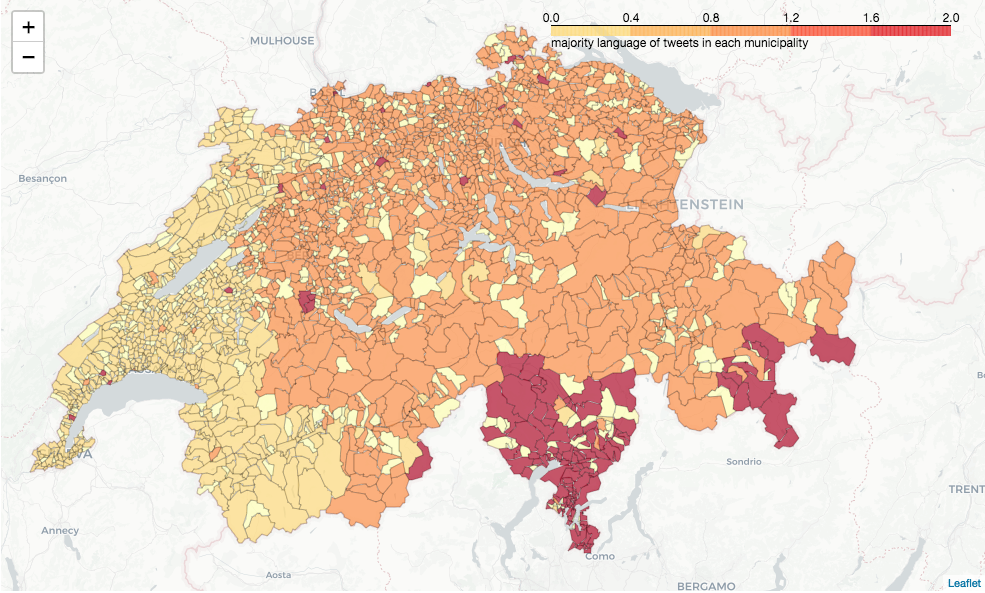
\includegraphics[width=0.5\textwidth]{images/rosti_map.png}
  \caption{The R\"ostigraben reconstructed from the language of the tweets. The color encoding is yellow: French; orange: German, red: Italian}
  \label{rosti_map}
\end{figure}

\begin{figure}[h]
  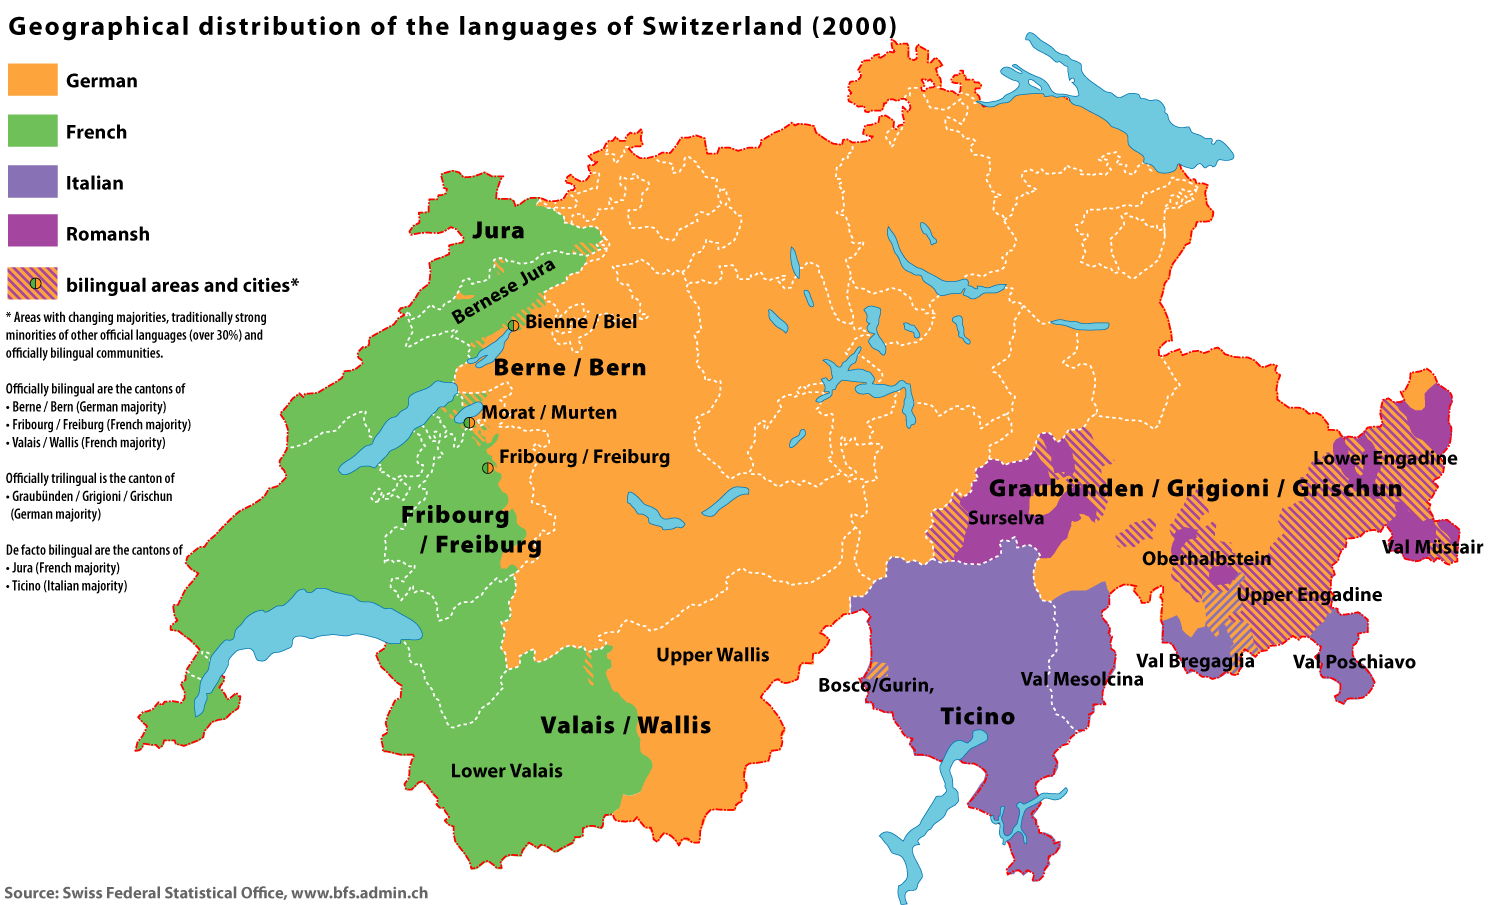
\includegraphics[width=0.5\textwidth]{images/Map_Languages_CH.png}
  \caption{The R\"ostigraben from its Wikipedia page (originally from admin.ch)}
  \label{rosti_map_wiki}
\end{figure}

\subsection{Political activity}

TODO: Ramtin 
